\documentclass[sigconf]{acmart}

\usepackage{booktabs}
\usepackage{algorithm,algorithmic}
\usepackage{dsfont}
\usepackage{multirow}
\usepackage[english]{babel}
\graphicspath{ {images/} }

\def\ind{\mathds{1}}
\def\E{\mathbb{E}}
\def\P{\mathbb{P}}
\def\Cov{\mathrm{Cov}}
\def\Var{\mathrm{Var}}
\def\deg{\mathrm{deg}}
\def\cV{\mathcal{V}}
\def\cN{\mathcal{N}}
\def\co{\mathrm{co}}

\newcommand\independent{\protect\mathpalette{\protect\independenT}{\perp}}
\def\independenT#1#2{\mathrel{\rlap{$#1#2$}\mkern2mu{#1#2}}}

\def\myplotwidth{0.23\textwidth}

\usepackage{lipsum}

% Copyright
%\setcopyright{none}
%\setcopyright{acmcopyright}
%\setcopyright{acmlicensed}
\setcopyright{rightsretained}
%\setcopyright{usgov}
%\setcopyright{usgovmixed}
%\setcopyright{cagov}
%\setcopyright{cagovmixed}

% DOI
\acmDOI{10.475/123_4}

% ISBN
\acmISBN{123-4567-24-567/08/06}

%Conference
\acmConference[KDD'18]{KDD conference}{August 2018}{London, UK}
\acmYear{2018}
\copyrightyear{2018}

\acmArticle{4}
\acmPrice{15.00}

\begin{document}
\title{Estimating Graphlet Statistics via Lifting}

\author{Kirill Paramonov}
\affiliation{
    \institution{University of California, Davis}
    \streetaddress{One Shields Ave.}
    \postcode{95616}
}
\email{kir.paramonov@gmail.com}


\author{James Sharpnack}
\affiliation{
    \institution{University of California, Davis}
    \streetaddress{One Shields Ave.}
    \postcode{95616}
}
\email{jsharpna@gmail.com}

\begin{abstract}
    Exploratory analysis over network data is often limited by our ability to efficiently calculate graph statistics, which can provide a model-free understanding of macroscopic properties of a network.
    %such as the clustering coefficient, algebraic connectivity, and network diameter.
    This work introduces a framework for estimating the graphlet count---the number of occurrences of a small subgraph motif (e.g. a wedge or a triangle) in the network.
	For massive graphs, where accessing the whole graph is not possible, the only viable algorithms are those which act locally by making a limited number of vertex neighborhood queries.
    We introduce a Monte Carlo sampling technique for graphlet counts, called {\em lifting}, which can simultaneously sample all graphlets of size up to $k$ vertices.
    We outline three variants of lifted graphlet counts: the ordered, unordered, and shotgun estimators. 
%	the only option is to have an on-line learning procedure while travelling from vertex to vertex, and gather information about the local structure of the graph.
	We prove that our graphlet count updates are unbiased for the true graphlet count, have low correlation between samples, and have a controlled variance.
	We compare the experimental performance of lifted graphlet counts to the state-of-the art graphlet sampling procedures: Waddling and the pairwise subgraph random walk.
	
%	Extracting data from social networks becomes more and more important because of the wide applicability of such algorithms.
% 	For the large graphs (like Facebook), where the access to the whole graph is not possible, the only option is to have an on-line learning procedure while travelling from vertex to vertex, and gather information about the local structure of the graph.
% 	An important local statistic of a network is graphlet count- the number of occurrences of a small motif (e.g. a wedge or a triangle) in the big network.
	
% 	In this paper, we propose a new Lifting algorithm to construct an estimate of the graphlet count statistic, which has an advantage of having low correlation between samples and being universal for all types of graphlets.
% 	We also propose several modifications for the algorithm: Ordered Lifting, Shotgun Lifting and Unordered Lifting, with each modification being more applicable to a specific goal, making the estimator that much versatile for different problems.
	
% 	We also demonstrate the improvement in accuracy and variation compared to state-of-art algorithms when applied to many different real-world networks.
\end{abstract}

%
% The code below should be generated by the tool at
% http://dl.acm.org/ccs.cfm
% Please copy and paste the code instead of the example below.
%
% \begin{CCSXML}
% <ccs2012>
%  <concept>
%   <concept_id>10010520.10010553.10010562</concept_id>
%   <concept_desc>Computer systems organization~Embedded systems</concept_desc>
%   <concept_significance>500</concept_significance>
%  </concept>
%  <concept>
%   <concept_id>10010520.10010575.10010755</concept_id>
%   <concept_desc>Computer systems organization~Redundancy</concept_desc>
%   <concept_significance>300</concept_significance>
%  </concept>
%  <concept>
%   <concept_id>10010520.10010553.10010554</concept_id>
%   <concept_desc>Computer systems organization~Robotics</concept_desc>
%   <concept_significance>100</concept_significance>
%  </concept>
%  <concept>
%   <concept_id>10003033.10003083.10003095</concept_id>
%   <concept_desc>Networks~Network reliability</concept_desc>
%   <concept_significance>100</concept_significance>
%  </concept>
% </ccs2012>
% \end{CCSXML}

% \ccsdesc[500]{Computer systems organization~Embedded systems}
% \ccsdesc[300]{Computer systems organization~Redundancy}
% \ccsdesc{Computer systems organization~Robotics}
% \ccsdesc[100]{Networks~Network reliability}

% \keywords{ACM proceedings, \LaTeX, text tagging}
\maketitle


	\section{Introduction}
	\label{sec:intro}
	
    %Broad intro
    In 1970, \cite{davis1970clustering} discovered that transitivity---friends of friends tend to be friends themselves---is a prevalent feature in social networks.
    Since that early discovery, real-world networks have been observed to have many other common macroscopic features, and these discoveries have lead to probabilistic models for networks that display these phenomena.
    The observation that transitivity and other common subgraphs are prevalent in networks lead to the exponential random graph model \cite{frank1986markov}.
    \cite{barabasi1999emergence} demonstrated that many large networks display a scale-free power law degree distribution, and provided a model for constructing such graphs.
    Similarly, the small world phenomenon---that networks display surprisingly few degrees of separation---motivated the network model in \cite{watts1998collective}.
    While network science is often driven by the observation and modelling of common properties in networks, it is incumbent on the practicing data scientist to explore network data using statistical methods. 
    
    One approach to understanding network data is to fit free parameters in these network models to the data through likelihood-based or Bayesian methods. 
    In \cite{wasserman1996logit}, a pseudolikelihood method was used with graphlet counts to fit an ERGM designed to display transitivity, and Monte Carlo Markov Chain methods were developed in \cite{snijders2002markov} for fitting general ERGMs.
	Fitting such models from data can be cumbersome, and to do so implicitly assumes that the network follows such a model exactly.
	Network statistics, such as the clustering coefficient, algebraic connectivity, and degree sequence, are more flexible tools.
	A good statistic can be used to fit and test models, for example, \cite{watts1998collective} used the local clustering coefficient, a measure of the number of triangles relative to wedges, to test if a network is a small-world graph.
	The clustering coefficient is also used to understand social network graphs, \cite{chakrabarti2006graph}.
	More generally, it was discovered that re-occurring subgraph patterns can be used to differentiate real-world networks, and that genetic networks, neural networks, and internet networks all presented different common interconnectivity patterns, \cite{milo2002network}.
	In this work, we will propose a new method for counting the occurrences of any subgraph pattern, otherwise known as {\em graphlets}---a term coined in \cite{prvzulj2004modeling}---or motifs.
	
\begin{figure}[th]
\begin{center}
\hspace*{\fill}
\minipage{0.08\textwidth}
  
\includegraphics[width=\linewidth]{graphlet_2-1.png}
  \caption*{$H_1^{(2)}$}
\endminipage\hfill
\minipage{0.08\textwidth}
  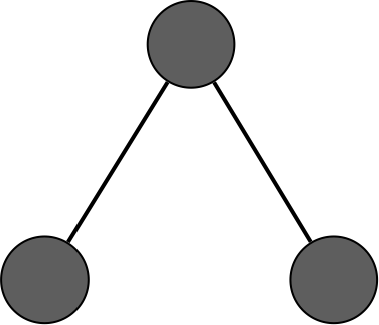
\includegraphics[width=\linewidth]{graphlet_3-1.png}
  \caption*{$H_1^{(3)}$}
\endminipage\hfill
\minipage{0.08\textwidth}
  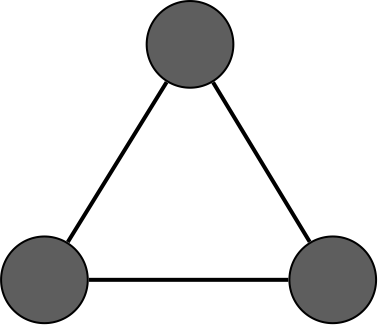
\includegraphics[width=\linewidth]{graphlet_3-2.png}
  \caption*{$H_2^{(3)}$}\label{}
\endminipage
\hspace*{\fill}
\vskip 5pt
\hspace*{\fill}
\minipage{0.06\textwidth}%
  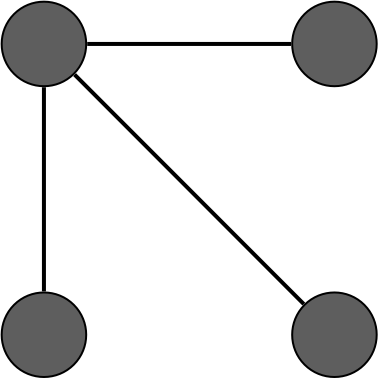
\includegraphics[width=\linewidth]{graphlet_4-1.png}
  \caption*{$H_1^{(4)}$}
\endminipage\hfill
\minipage{0.06\textwidth}
  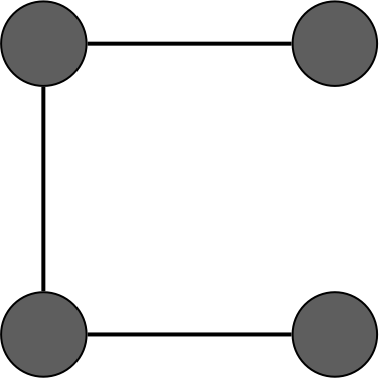
\includegraphics[width=\linewidth]{graphlet_4-2.png}
  \caption*{$H_2^{(4)}$}
\endminipage\hfill
\minipage{0.06\textwidth}
  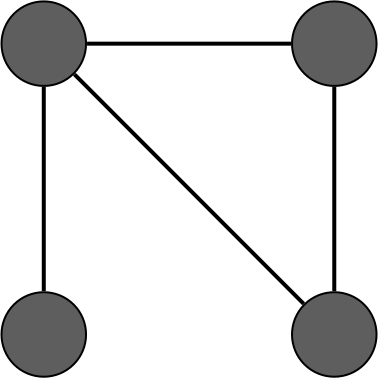
\includegraphics[width=\linewidth]{graphlet_4-3.png}
  \caption*{$H_3^{(4)}$}
\endminipage\hfill
\minipage{0.06\textwidth}
  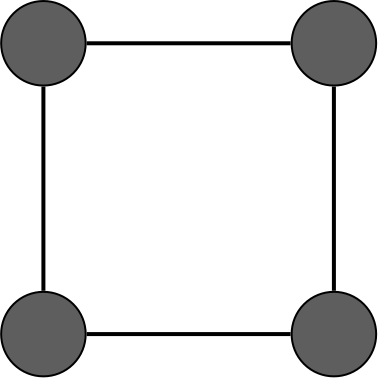
\includegraphics[width=\linewidth]{graphlet_4-4.png}
  \caption*{$H_4^{(4)}$}\label{}
\endminipage\hfill
\minipage{0.06\textwidth}%
  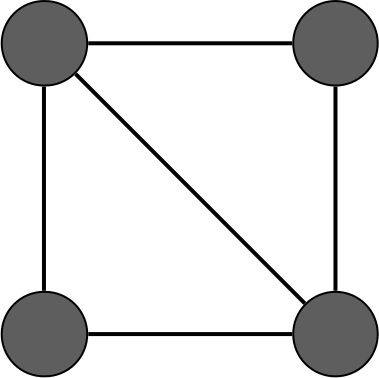
\includegraphics[width=\linewidth]{graphlet_4-5.png}
  \caption*{$H_5^{(4)}$}
\endminipage\hspace*{\fill}
\minipage{0.06\textwidth}%
  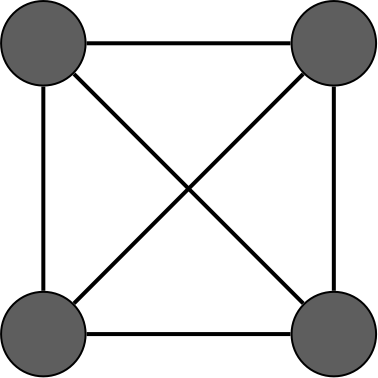
\includegraphics[width=\linewidth]{graphlet_4-6.png}
  \caption*{$H_6^{(4)}$}
\endminipage\hspace*{\fill}
\hspace*{\fill}
\vskip 5pt
\hspace*{\fill}
\minipage{0.08\textwidth}%
  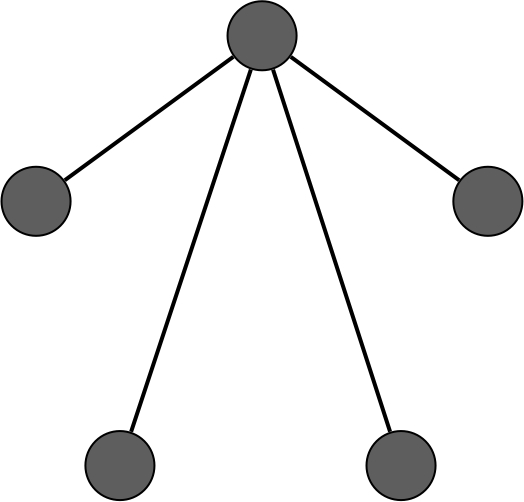
\includegraphics[width=\linewidth]{graphlet_5-1.png}
  \caption*{$H_1^{(5)}$}
\endminipage\hfill
\minipage{0.08\textwidth}
  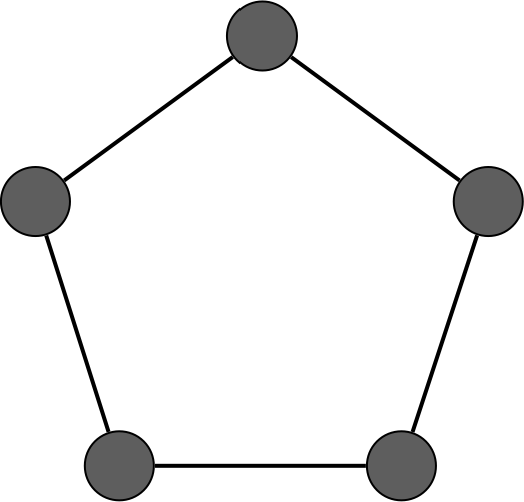
\includegraphics[width=\linewidth]{graphlet_5-8.png}
  \caption*{$H_8^{(5)}$}
\endminipage\hfill
\minipage{0.08\textwidth}
  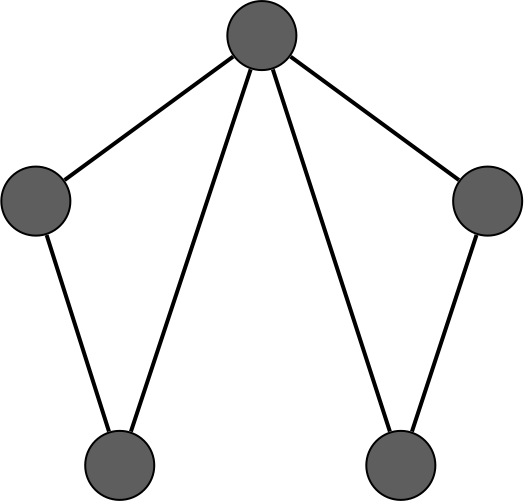
\includegraphics[width=\linewidth]{graphlet_5-11.png}
  \caption*{$H_{11}^{(5)}$}
\endminipage\hfill
\minipage{0.08\textwidth}
  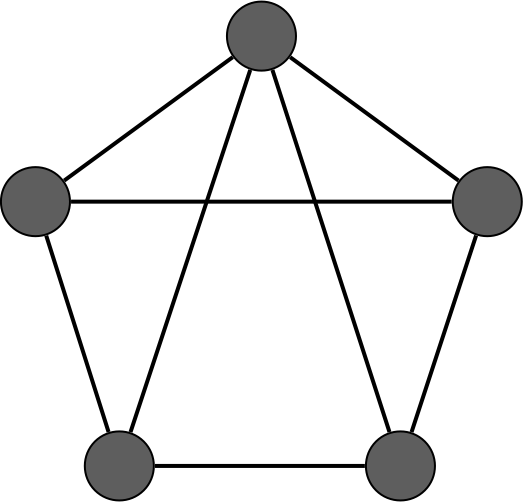
\includegraphics[width=\linewidth]{graphlet_5-19.png}
  \caption*{$H_{19}^{(5)}$}\label{}
\endminipage\hfill
\minipage{0.08\textwidth}%
  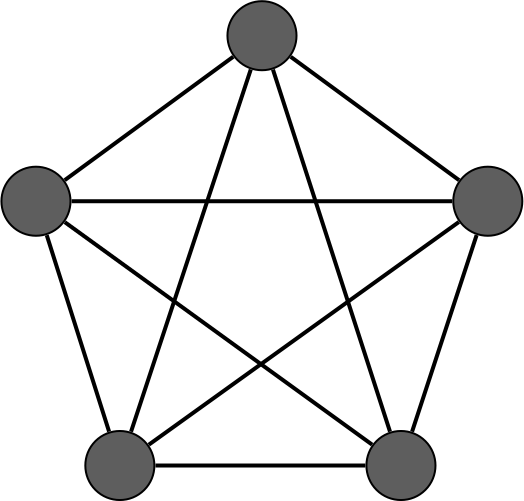
\includegraphics[width=\linewidth]{graphlet_5-21.png}
  \caption*{$H_{21}^{(5)}$}
\endminipage\hspace*{\fill}
\caption{Examples of graphlets}
\label{fig:graphlets}
\end{center}
\end{figure}

	
	%Intro to graphlets
	A graphlet is a small graph topology, such as a triangle, wedge, or $k$-clique, which we will use to describe the local behavior of a larger network (example graphlets of size 3, 4, and 5, can be seen in Figure \ref{fig:graphlets}).
	Let the graph in question be $G = (V,E)$ where $V$ is a set of vertices and $E$ is a set of unordered pairs of vertices ($G$ is assumed to be undirected).
	Imagine specifying a $k$-graphlet and testing for every induced subgraph of the graph (denoted $G|\{v_1,\ldots,v_k\}$ where $v_1,\ldots,v_k \in V$), if it is isomorphic (has the same topology) to the subgraph.
	We would like to compute the number of subgraphs for which this match holds, and the proportion of the number of such matches to the number of connected induced subgraphs of that size is called the {\em graphlet coefficient}.
	
    Graphlets are the graph analogue of wavelets (small oscillatory functions that are convolved with a signal to produce wavelet coefficients) because they are small topologies that are matched to induced subgraphs of the original graph to produce the graphlet coefficients.
	Graphlet coefficients, also referred to as graph moments, are used in the method of moments to fit certain graph models by selecting parameters that match the empirical graph moments to their expectations \cite{bickel2011method}.
	Graphlet coefficients are used to understand biological networks, such as the protein-protein interaction network, and reoccuring patterns are thought to indicate evolutionary conserved modules \cite{prvzulj2006efficient}. 
	If $k$ is small then testing for isomorphism, a problem called graph matching \cite{cordella2004sub}, is feasible, but testing every induced subgraph can require on the order of $n^k$ iterations in its most naive implementation.
	We propose a class of methods called lifting methods that allow us to quickly estimate graphlet coefficients.

	%Graphlet sampling
	
	While there exist several algorithms that can estimate the proportion of triangles, wedges, and graphlets with four or five vertices (for eaxample, \cite{Ahmed2017count, rahman2014graft}), there are few algorithms that can efficiently estimate the proportion of larger graphlets.
	Many methods that can handle arbitrary graphlets are Monte Carlo sampling procedures that traverse through the space of all subgraphs of a certain size.
	Two such methods are GUISE algorithm of \cite{bhuiyan2012guise}, the pairwise subgraph random walk of \cite{Wang2014psrw}, and the Waddling random walk of \cite{Han2016waddling}, which differ in the way that they perform a random walk between the induced subgraphs.
	Alternatives to Monte Carlo schemes include the color coding scheme of \cite{Bressan2017colourcoding}, but it processes the whole graph, while the Monte Carlo schemes can traverse the network locally.
    In this work, we propose a new Monte Carlo algorithm, called lifting, for estimating the graphlet frequencies within a large network.
    The lifting step takes a smaller subgraph of size $k-1$ and produces a subgraph of size $k$ by adding an adjacent vertex to it (according to a specific scheme).  
    In this paper we consider procedures that start from vertices or edges and lift to sample subgraphs of size $k$.
	Lifting is a simple, flexible procedure that can be easily distributed to accommodate massive network datasets.
	
	\subsection{Our contributions}
	
	Graphlet coefficients are multipurpose statistical tools that can be used for model fitting and testing, network regression, and exploratory analysis for network data.
    Any subgraph Monte Carlo sampling scheme has three goals: that it provides unbiased estimates of the graphlet coefficients, that the variance of the estimated coefficients is small, and that it does so in as few iterations as possible.
    Because massive graphs are often stored in distributed databases, we would like the sampling scheme to require only neighborhood queries (requests to the database returns the neighbors of a node) and we will avoid storing or processing the full graph.
    Because communication is often the bottleneck in distributed computing, neighborhood queries are the basic unit for measuring computational time complexity.
    
    After discussing the precise requirements for any graphlet sampling procedure, we will introduce the lifting scheme for graphlets.
    The key difficulty in any Monte Carlo method for graphlet coefficient is calculating the sampling distribution.
    We provide two methods, the ordered lift estimator and the unordered lift estimator, which differ in the way that subgraphs are represented and counted in the graphlet coefficient.
    The ordered estimator allows for a modification, called {\em shotgun sampling} that samples multiple graphlets in one shot. 
    For our theoretical component, we prove that the estimated graphlet coefficients are unbiased when the underlying MCMC has reached the stationary distribution (called perfect mixing).
    We also prove that under perfect mixing, the variance of the estimator scales like $\Delta^{k-2}$ where $\Delta$ is the maximum degree, and show that the lifting scheme can have significantly lower mixing rates than the subgraph random walk.
    We conclude with real-world network experiments that reinforce the contention that graphlet lifting has a lower variance and better mixing rates than subgraph random walks.

	\section{Estimating graphlet frequencies via sampling}

	\subsection{Definitions and notation}
	
	Consider graph $G=(V,E)$ with set of vertices $V$ and set of edges $E \subseteq
	\binom{V}{2}$. 
	We assume $G$ to be simple, connected and undirected. 
	(It's easy to translate our results to the case of directed graphs, since we will mostly be 
	focusing on sampling procedure.) 
	For a subset $W \subseteq V$, a subgraph of $G$ induced 
	by $W$, $G|W$ is a graph with vertices in $W$ and edges in $\binom{W}{2}\cap E$. 
	If $|W| = k$ and $G|W$ is connected, then we say that $G|W$ is a $k$-subgraph of 
	$G$. The set of all $k$-subgraphs of $G$ is denoted by $\cV_k(G)$ (or simply $\cV_k$).
	Given a $k$-graphlet, $H$, (a graph on $k$ nodes), we'll be interested in the number 
	of $k$-subgraphs of $G$ isomorphic to $H$.
	
	We'll make use of Python notation for lists vs sets: if we don't need indices or respective
	ordering of elements, we'll write it as a set $\{v_1, \ldots, v_k\}$, and if the 
	order of the elements is fixed or indices are used to distinguish the elements, we'll write 
	it as a list $[v_1,\ldots, v_k]$. 
	Let $Gr_k = [H_1, H_2, \ldots, H_l]$ be the list of all non-isomorphic
	connected $k$-graphlets. For $T\in \cV_k(G)$, we say that ''$T$ is graphlet of
	 type $m$'' if $T$ is isomorphic to $H_m$. Notation: $T \sim H_m$.
	
	The number of $k$-graphlets of $G$ of type $m$ is equal to 
	$N_m (G) = \sum_{T \in \cV_k(G)} \ind(T \sim H_m)$, where $\ind(A)$ 
	is the indicator function of boolean $A$.

    \subsection{Monte Carlo estimation of graphlet frequencies}
	
	    Monte Carlo Markov Chains (MCMC) typically start from an initial distribution that then converges to the stationary distribution.
    A requirement 

    The ideal Monte Carlo procedure would sequentially sample graphlets uniformly at random from the set of all graphlets within $G$, classify their type, and update the corresponding moments.  
Unfortunately, uniformly sampling graphlets is not a simple task because they are required to be connected---a random set of k vertices is unlikely to be connected.
We turn to Markov chains to sample more effectively.
First, let us consider how we update the graph moments, $N_m(G)$, given a sample of graphlets $T_1, T_2, \ldots, T_n$.

The desire to sample graphlets uniformly is natural, because the empirical moments will be unbiased estimates of the graph moments.
Suppose that each graphlet, $T_i$, is drawn from the common distribution $\pi$ over the space of graphlets.
Then we use Horvitz-Thompson inverse probability weighting to estimate the graph moments,
\begin{equation}
  \label{eq:moments}
  \hat N_m(G) := \frac{1}{n} \sum_{i=1}^n \frac{\ind(T_i\sim H_m)}{\pi(T_i)}.  
\end{equation}
It is simple to see that this is an unbiased estimate of the moments as long as $\pi$ is supported over all k-graphlets.
We find ourselves in a game, where we can choose any graphlet Monte Carlo algorithm that induces a stationary distribution $\pi$, but we must be able to quickly and accurately compute $\pi$ in order to use \eqref{eq:moments}.
We will analyze the theoretical implications of the sampling algorithm based on mixing times of the Markov chain and the variance of the moment estimates in Section ??.

\subsection{Subgraph random walk}

Before we explore the lifting procedure, this paper's algorithmic contribution, we would like to discuss some existing Monte Carlo graphlet sampling methods.
Any admissible graphlet Markov chain transitions between k-graphlets of $G$ and the transition probabilities have a calculable stationary distribution $\pi$.
The basic algorithm is listed in \ref{alg:SRW}, and some elements are left purposefully vague to maintain generality.
Many of the proposed graphlet sampling algorithms can be encompassed by this master algorithm, and we will highlight the two most prominent examples: Subgraph random walk and waddling random walk.

\begin{algorithm}
\label{alg:SMC}
\caption{Subgraph Markov chain}
\begin{algorithmic}
  \STATE Initialize $T$ at an arbitrary k-graphlet, $n \gets 1$, $\hat N_m(G) \gets 0$
  \WHILE{stopping criteria is not met}
  \STATE Query the neighbors of each vertex in $T$, $\{\mathcal N (v): v \in T\}$
  \STATE Add a vertex according to an {\em add rule}
  \STATE Remove a vertex according to a {\em remove rule}
  \IF{{\em Markov chain is sufficiently mixed}}
  \STATE Determine the type $m$ of $T$, calculate $\pi(T)$
  \STATE Update $\hat N_m(G) \gets ((n -1) \hat N_m(G) + \pi^{-1}(T))/n$ and $n \gets n + 1$
  \ENDIF
  \ENDWHILE
\end{algorithmic}
\end{algorithm}

Mixing is a critical issue for any Markov chain based sampling, and graphlet sampling is no exception.
We will mathematically define mixing in Section ??, but, in words, it measures the dependence between consecutive samples.
Dependence between consecutive samples results in a higher variability of $\hat N_m(G)$, and because calculating $\pi(T)$ and determining the type of $T$ can be computationally cumbersome, it is advisable to not include every subgraph in the final sample.
One easy way to achieve this is to sample only every several iterations, where the sampling frequency is calibrated to obtain a certain level of mixing.

\noindent{\bf Subgraph random walk.}


{\bf }

\subsection{Lifting procedures}

    This approach gives an unbiased estimator assuming $\pi_k(T) >0$ for any $T\in \cV_k$.
    The biggest issue of this method is the variance of $\hat N_m(G)$. We rewrite the variance as a sum of two terms:
	\begin{multline}
	\label{eq:variation}
		\Var(\hat N_m(G)) = \frac{1}{n}\left( \E_{\pi_k} \frac{\ind(T\sim H_m)}{\pi_k(T)^2} - N_m^2(G)\right) +\\
		\frac{2}{n^2} \sum_{i < j} \Cov_{\pi_k}\left( \frac{\ind(T_i\sim H_m)}{\pi_k(T_i)}, \frac{\ind(T_j\sim H_m)}{\pi_k(T_j)}\right).
	\end{multline}
	
	The first term will be referred to as variation under independence term, and can dominate the sum if $\pi_k(T)$ greatly deviates from the uniform probability $\rho(T) = \frac{\ind(T\sim H_m)}{N_m(G)}$.
	The second term will be referred to as a covariance term and can dominate the sum when graphlets $T_i$ and $T_{i+1}$ have high correlation, which is the case for Subgraph Random Walk methods discussed below.
	
	The previous papers on that topic focused on efficient method of sampling a sequence of $k$-graphlets, depending on a framework.
	We'll try to summarize the frameworks and corresponding methods here.
	
	There are two different frameworks, each with its own problem statement.
	\begin{itemize}
		\item \textbf{Framework 1.} We have access to the whole graph structure, for example, in the form of adjacency matrix. 
		We can sample the nodes of the graph cheaply, independently and according to an arbitrary probability distribution.
		The goal is to sample graphlets quickly, uniformly and independently.
		In particular, the covariance term would be irrelevant in this framework.
		The state-of-art method for this framework is Color Coding \cite{Bressan2017colourcoding}.

		\item \textbf{Framework 2.} We start with an access to a single node $v_0$ and its 
		neighborhood. As a query, we can transition to a neighboring node $v_1$ and get access to the neighborhood of $v_1$.
		Each moment of time we can only get access to the neighbors of previously visited nodes. 
		This framework is applied when queries are either expensive or limited and traversing the whole graph is time-prohibitive at best and not feasible at worst. 
		The goal here is to achieve best accuracy with either limited number of queries ($10^3-10^4$ queries for graphs with $10^5-10^6$ nodes) or limited time, or something in between (costly queries).
		Recent methods include Subgraph Random Walk(SRW) and Pairwise Random Walk \cite{Wang2014psrw} and Waddling Random Walk (WRW) \cite{Han2016waddling}.
	\end{itemize}
	
	For each of the two frameworks above we'll present a modification of the base algorithm
	to suit corresponding goals.
	
	\subsection{Subgraph Random Walk (SRW)}
	For this method, consider a set $\mathcal{G}_k$ of all $k$-graphlets of $G$.
	We introduce graph structure on $\mathcal{G}_k$ by connecting two graphlets $T,S \in \mathcal{G}_k$ with an edge if and only if vertex sets of $T$ and $S$ differ by one element, i.e. when $|V(T) \cap V(S)| = k-1$.
	Given the graph structure, we sample $k$-graphlets by random walk on the set of vertices $\mathcal{G}_k$, which is called Subgraph Random Walk (SRW).
	It was pointed out in \cite{Bressan2017colourcoding} that the mixing time of the SRW can be of order $O(n^{k-2})$, even if the mixing time of the random walk on the original graph $G$ is of constant order $O(1)$.
	Thus, it would require $O(n^{k-2})$ burn-in steps to get uncorrelated samples from SRW.
		
	
	\section{Algorithm Description (to be merged with above)}
	\subsection{Lifting procedure}
	
	For a subgraph $S \subseteq G$, denote $V_S$ to be the set of its vertices, $E_S$ to be the set of its edges.
	Denote $\cN_v(S)$ (vertex neighborhood of $S$) to be the set of all vertices adjacent to some vertex in $S$ not including $S$ itself. 
	Denote $\cN_e(S)$ (edge neighborhood of $S$) to be the set of all edges that connect a vertex from $S$ and a vertex outside of $S$.
	Formally,
	\begin{equation*}
		\cN_v(S) = \{u\in V_G\setminus V_S \mid \exists s\in V_S : (s,u)\in E_G\},
	\end{equation*}
	\begin{equation*}
		\cN_e(S) = \{(s,u)\in E_G \mid s\in V_S, u\notin V_S\}.
	\end{equation*}	
	
	Denote $\deg(S)$ (degree of $S$) to be the number of edges in $\cN_e(S)$, and denote $\deg_S(u)$ ($S$-degree of $u$) to be the number of vertices from $S$ that are connected to $u$.
	Formally,
	\begin{equation*}
		\deg(S) = |\{(s,u)\in E_G \mid s\in V_S, u\notin V_S\}|,
	\end{equation*}
	\begin{equation*}
		\deg_S(u) = |\{s\in V_S\mid (u,s)\in E_G\}|.
	\end{equation*}
	Note that $\deg(S) + 2|E_S| = \sum_{v\in V_S} \deg(v)$.
	
	First assume we have a node $v_1$ sampled from the distribution $\pi_1$ (we will address this assumption later). 
	We also assume that $\pi_1(v) = \frac{f(\deg(v))}{K}$, where $f(x)$ is some function (usually a polynomial) and $K$ is some global normalizing constant.
	Denote $S_1 = \{v_1\}$.

\begin{figure}[th]
\begin{center}
\hspace*{\fill}
\minipage{0.10\textwidth}
  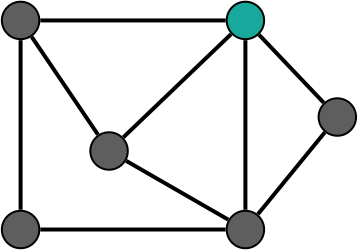
\includegraphics[width=\linewidth]{lift_1.png}
  \caption*{(a)}
\endminipage\hfill
\minipage{0.10\textwidth}
  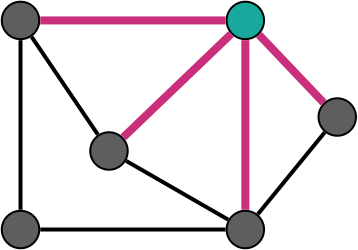
\includegraphics[width=\linewidth]{lift_2.png}
  \caption*{(b)}
\endminipage\hfill
\minipage{0.10\textwidth}
  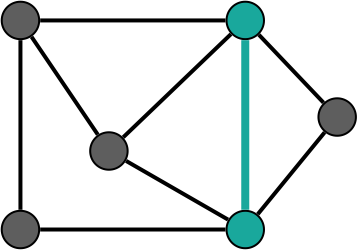
\includegraphics[width=\linewidth]{lift_3.png}
  \caption*{(c)}\label{}
\endminipage\hfill
\minipage{0.10\textwidth}%
  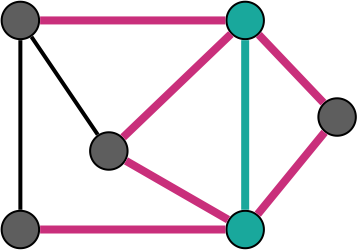
\includegraphics[width=\linewidth]{lift_4.png}
  \caption*{(d)}
\endminipage
\hspace*{\fill}
\vskip 5pt
\hspace*{\fill}
\minipage{0.10\textwidth}
  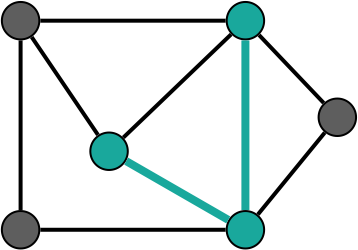
\includegraphics[width=\linewidth]{lift_5.png}
  \caption*{(e)}
\endminipage\hfill
\minipage{0.10\textwidth}
  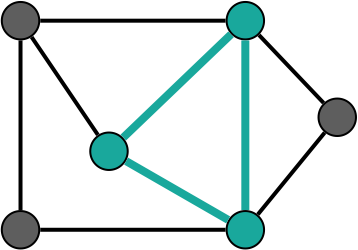
\includegraphics[width=\linewidth]{lift_6.png}
  \caption*{(f)}
\endminipage\hfill
\minipage{0.10\textwidth}
  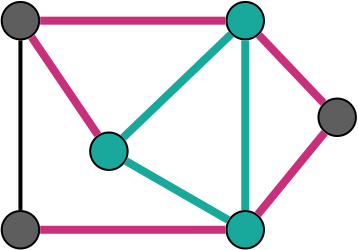
\includegraphics[width=\linewidth]{lift_7.png}
  \caption*{(g)}\label{}
\endminipage\hfill
\minipage{0.10\textwidth}%
  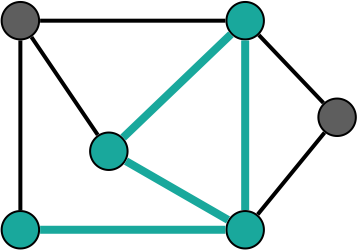
\includegraphics[width=\linewidth]{lift_8.png}
  \caption*{(h)}
\endminipage\hspace*{\fill}
\caption{Lifting procedure}
\end{center}
\end{figure}

	To start our procedure, sample an edge $(v_1,v_2)$ uniformly from $\cN_e(S_1)$. 
	The vertex $v_2$ is then attached to $S_1$, forming a subgraph $S_2 = G|(V_{S_1} + {v_2})$.
	After that, we sample another edge $(v_i, v_3)$ (with $1\leq i\leq 2$) uniformly from $\cN_e(S_2)$, and the vertex $v_3$ is then attached to $S_2$.
	
	Generally, sample an edge $(v_i, v_{r+1})$ (with $1\leq i \leq r$) from $\cN_e(S_r)$ uniformly at random, and attach the vertex $v_{r+1}$ to the subgraph $S_r$.
	After $k-1$ operations, we obtain a $k$-graphlet $T = S_k$.
	
	We'll refer to the procedure above as the \textbf{lifting} procedure starting at vertex $v_1$.
	
	Using the lifting procedure, we can get two estimators of the graphlet count statistic.
	
	\subsection{Ordered lift estimator}
	
	We can think of a lifting procedure as a way of sampling a sequence $A = [v_1, \ldots, v_k]$ that is then used to generate a graphlet.
	Denote the set of such sequences as $V^k_G$.
	For $A = [v_1, \ldots, v_k] \in V^k_G$, denote $A[i]:=v_i$.
	Let $S_r = S_r(A) = G|\{v_1,\ldots, v_r\}$ be the $r$-graphlet obtained by the lifting procedure on step $r$.
	The probability of sampling vertex $v_{r+1}$ on the step $r+1$ is equal to
	\begin{equation*}
	    \mathbb{P}(v_{r+1}|S_{r}) := \frac{\deg_{S_r}(v_{r+1})}{|\cN_e(S_r)|} =
	    \frac{|E_{S_{r+1}}| - |E_{S_r}|}{\sum_{i=1}^r \deg(v_i) - 2|E_{S_r}|}.
	\end{equation*}
	THIS IS KEY STEP.
	Thus, the probability of sampling a sequence $A \in V^k_G$ is equal to
	\begin{multline}
	\label{eq:tildepi}
	    \Tilde\pi_k(A) := \pi_1(A[1])\prod_{r=1}^{k-1} \P\left(A[r+1]|S_r(A)\right) =\\
	    \frac{f(\deg(A[1]))}{K} \prod_{r=1}^{k-1} \frac{|E_{S_{r+1}(A)}| - |E_{S_r(A)}|}{\sum_{i=1}^r \deg(A[i]) - 2|E_{S_r(A)}|}.
	\end{multline}
	Consider the sampled $k$-graphlet $T := S_k(A)$.
	Denote the set of possible sequences $A = [v_1,\ldots, v_k]$ that would form a graphlet $T$ in the lifting process as $\co(T)$.
	Notice that $S_r(A) = G|\{v_1,\ldots,v_r\} = T|\{v_1,\ldots,v_r\}$ must be a connected subgraph for all $r$.
	Thus,
	\begin{multline}
	\label{eq:co}
	    \co(T) = \big\{\,[v_1,\ldots,v_k]\in V^k_G \mid \{v_1,\ldots,v_k\} = V_T,\\  T|\{v_1,\ldots,v_r\} \text{ is connected }\big\}.
	\end{multline}
	Since the elements of $\co(T)$ are just certain orderings of vertices in $T$, we call an element from $\co(T)$ a \textit{compatible ordering} of $T$.
	Note that $|\co(T)|$ only depends on the type of the graphlet $T$.
	Thus, when $T\sim H_m$, the number of compatible orderings are equal: $|\co(H_m)| = |\co(T)|$. Note that $|\co(H_m)|$ can vary from $2^{k-1}$ (for $k$-path) to $k!$ (for $k$-clique).
	
	Next, we set up the expectation:
	\begin{multline*}
	    \frac{1}{|\co(H_m)|}\E_{\tilde \pi_k} \frac{\ind\left(T \sim H_m\right)}{\tilde\pi_k([v_1, \ldots, v_k])} = 
	    \sum_{[v_1, \ldots, v_k]} \frac{\ind(T \sim H_m)}{|\co(T)|} = \\
	    \sum_T \ind(T \sim H_m) = N_m(G).
	\end{multline*}
	The empirical expectation of the value on the left-hand side gives an estimate for $N_m(G)$.
	Let $A_1,\ldots,A_n$ be sequences from $V^k_G$ sampled in the lifting process.
	Then
	\begin{equation*}
	    \frac{1}{n}\frac{1}{|\co(H_m)|}\sum_{i} \frac{\ind(G|A_i \sim H_m)}{\tilde\pi_k(A_i)} \approx N_m(G).
	\end{equation*}
	We call that estimator an \textit{ordered lift estimator} for graphlet count statistic.
	
\begin{algorithm}[h]
\label{alg:OLE}
\caption{Ordered Lift Estimator (with optional shotgun sampling)}
\begin{algorithmic}
    \INPUT Graph $G$, $k$-graphlet $H_m$
    \OUTPUT $\hat N_m(G)$
    \STATE Count $|\co(H_m)|$- the number of compatible orderings in $H_m$.
    \STATE Initialize $v$ at an arbitrary node, $n \gets 0$, $\hat N_m(G) \gets 0$
    \WHILE{stopping criteria is not met}
        \STATE Sample $v_1$ from $\pi_1(v)$
        \STATE Initialize $V_S \gets \{v_1\}$ and $E_S \gets \{\}$
        \STATE Initialize $\cN_e(S)\gets \cN_e(v_1)$
        \STATE Initialize $\pi(S) \gets \pi_1(v_1)$
        \WHILE{$|V_S| < k-1$}
            \STATE Sample an edge $e=(v,u)$ uniformly from $\cN_e(S)$, with $v\in V_S$ and $u\notin V_S$
            \STATE Set $E_S(u) \gets \{(v,u)\in \cN_e(S)\}$
            \STATE Update $\pi(S)\gets \pi(S)\frac{|E_S(u)|}{\sum_{v\in V_S} \deg(v) - 2|E_S|}$
            \STATE Update $V_S\gets V_S\cup\{u\}$ and $E_S \gets E_S \cup E_S(u)$
            \STATE Query $\cN_e(u)$
            \STATE Update $\cN_e(S) \gets [\cN_e(S)\cup\cN_e(u)]\setminus E_S(u)$
        \ENDWHILE
        \IF {not shotgun sampling}
            \STATE Sample an edge $e=(v,u)$ uniformly from $\cN_e(S)$, with $v\in V_S$ and $u\notin V_S$
            \STATE Set $E_S(u) \gets \{(v,u)\in \cN_e(S)\}$
            \STATE Set $\pi(T)\gets \pi(S)\frac{|E_S(u)|}{\sum_{v\in V_S} \deg(v) - 2|E_S|}$
            \STATE Set $V_T\gets V_S\cup\{u\}$ and $E_T \gets E_S\cup E_S(u)$
            \IF {$(V_T, E_T) \sim H_m$}
                \STATE Update $\hat N_m(G) \gets \hat N_m(G) + \pi^{-1}(T)$ 
            \ENDIF
        \ENDIF
        \IF {shotgun sampling}
            \FORALL{$u\in \cN_v(S)$}
                \STATE Set $E_S(u) \gets \{(v,u)\in \cN_e(S)\}$
                \STATE Set $V_T\gets V_S\cup\{u\}$ and $E_T \gets E_S \cup E_S(u)$
                \IF{$(V_T, E_T) \sim H_m$}
                    \STATE Update $\hat N_m(G) \gets \hat N_m(G) + \pi^{-1}(S)$
                \ENDIF
            \ENDFOR
        \ENDIF
        \STATE Update $n \gets n + 1$
    \ENDWHILE
    \STATE Normalize $\hat N_m(G) \gets \frac{1}{n}\frac{1}{|\co(H_m)|}\hat N_m(G)$
\end{algorithmic}
\end{algorithm}
	
	A drawback of the algorithm is that it takes $k-1$ queries to lift the graphlet plus the number of steps required to sample the first vertex (when sampled from Markov chain). 
	To increase the number of samples per query, notice that if we sample $B = [v_1, \ldots, v_{k-1}]$ via lifting, we can get graphlets induced by $A = [v_1,\ldots, v_{k-1},u]$ for all $u \in \cN_v(B)$ without using any additional queries:
	\begin{multline*}
	    N_m(G) = \frac{1}{|\co(H_m)|}\sum_{A} \ind(G|A \sim H_m) =\\
	    \frac{1}{|\co(H_m)|}\sum_{B}\sum_{u\in \cN_v(B)} \frac{\ind\left(G|(B+u) \sim H_m\right)}{\tilde\pi_{k-1}(B)} \tilde\pi_{k-1}(B) = \\
	    =\frac{1}{|\co(H_m)|} \E_{\tilde\pi_{k-1}} \frac{\sum_{u\in \cN_v(B)} \ind\left(G|(B+u) \sim H_m\right)}{\tilde\pi_{k-1}(B)}
	\end{multline*}
	Let $B_1,\ldots,B_n$ be sequences sampled from $V^{k-1}_G$ via lifting process.
	Then
	\begin{equation*}
	    \frac{1}{n}\frac{1}{|\co(H_m)|}\sum_{i=1}^n \frac{\sum_{u\in \cN_v(B_i)} \ind\left(G|(B_i+u)\sim H_m\right)}{\tilde\pi_{k-1}(B_i)} \approx N_m(G),
	\end{equation*}
	where we only make queries to the vertices of $B_i$.
	We call this technique \textbf{shotgun sampling}.
	
	Shotgun sampling is useful in cases when the number of queries is limited, but has a drawback of high correlation between samples.
	If the initial vertex $v_1$ was sampled from a random walk, the number of steps between initial vertices should be chosen so that shotgun shots are sufficiently far apart from each other.
	
	\subsection{Unordered lift estimator}
	
	We can also use the estimator \eqref{eq:moments} for the sampling space of $k$-graphlets $\cV_k(G)$.
	In order to do that, we need to compute the probability $\pi_k(T)$ of getting a particular $k$-graphlet $T \in \cV_k(G)$ in the lifting procedure.
	This can be done either recursively or directly. 
	Let the set of vertices of $T$ be $V_T=\{v_1,\ldots,v_k\}$.
	
	Recursive formula starts with known probabilities of initial vertices $\pi_1(v_i)$.
	Given a $k$-graphlet $T$, the probability of getting $T$ via lifting is given by the sum $\pi_k(T) = \sum_S \mathbb{P}(T|S) \pi_{k-1}(S)$, where the sum is taken over all $k-1$-subgraphlets $S\subset T$, and $\mathbb{P}(T|S)$ denotes the probability of getting from $S$ to $T$ in the lifting procedure.
	Let $T\setminus S$ be the unique vertex of $T$ that is not in $S$.
	Then
	\begin{multline}
	\label{eq:recursive}
		\pi_{k}(T) = \sum_{S\subset T} \pi_{k-1}(S) \frac{\deg_S (T\setminus S)}{|\cN_e(S)|} = \\
		\sum_{S\subset T} \pi_{k-1}(S) \frac{|E_T| - |E_S|}
		{\sum_{u\in S} \deg(u) - 2|E_S|},
	\end{multline}
	where the sum is taken over all $k-1$-subgraphlets $S\subset T$.
	
	For a direct formula, we notice that $\pi(T) = \sum_{A\in \co(T)} \tilde\pi(A)$, where $\co(T)$ is the set of compatible orderings of $T$ from previous section, and $\tilde\pi(A)$ is the probability of getting sequence $A\in \co(T)$ in the lifting process (see \eqref{eq:co},\eqref{eq:tildepi}).

	Then 
	\begin{equation}
	\label{eq:direct}
		\pi_k(T) = \sum_{A\in\co(T)} \frac{f(\deg(A[1]))}{K} \prod_{r=1}^{k-1} \frac{|E_{S_{r+1}(A)}| - |E_{S_r(A)}|}{\sum_{i=1}^r \deg(A[i]) - 2|E_{S_r(A)}|}
	\end{equation}
	
	Although calculation of that probability on-the-fly is cost-prohibitive, we can greatly reduce the number of operations by noticing that the probability $\pi_k(T)$ is a 
	function of degrees of the vertices: for a graphlet $T$ of type $m$, let $[v_1, \ldots, v_k]$ be the natural labelling of vertices in $T$ induced by the isomorphism $H_m \rightarrow T$ with $d_i = \deg(v_i)$, then the probability of $T$ is
	\begin{equation*}
	    \pi_k(T) =\frac{1}{K} F_m(d_1, \ldots, d_k)
	\end{equation*}
    for some cached function $F_m$.
	
	\textbf{Example.} Consider a triangle, which is a 3-graphlet with edges $(v_1,v_2)$, 
	$(v_2, v_3)$ and $(v_1,v_3)$. Given the degrees $d_1, d_2, d_3$ of the corresponding 
	vertices, the probability function is
	\begin{multline}
	\label{prob:triangle}
		\pi_3(\mathrm{triangle}) = \left( \frac{\pi_1(d_1)}{d_1} + 
		\frac{\pi_1(d_2)}{d_2}\right) \frac{2}{d_1+d_2-2} +\\ 
		+ \left( \frac{\pi_1(d_2)}{d_2} + \frac{\pi_1(d_3)}{d_3}\right) 
		\frac{2}{d_2+d_3-2} +\\
		\left( \frac{\pi_1(d_3)}{d_3} + \frac{\pi_1(d_1)}{d_1}\right) 
		\frac{2}{d_3+d_1-2}.
	\end{multline}
	
	\textbf{Example.} Consider a wedge, which is a 3-graphlet with edges $(v_1,v_2)$ and 
	$(v_1,v_3)$. Given the degrees $d_1, d_2, d_3$ of the corresponding 
	vertices, the probability function is
	\begin{multline}
	\label{prob:wedge}
		\pi_3(\mathrm{wedge}) = \left( \frac{\pi_1(d_1)}{d_1} + \frac{\pi_1(d_2)}{d_2}\right) \frac{1}{d_1+d_2-2} +\\
		\left( \frac{\pi_1(d_1)}{d_1} + \frac{\pi_1(d_3)}{d_3}\right) \frac{1}{d_1+d_3-2}.
	\end{multline}

	We need to only compute functions $F_m$ once before starting the algorithm.
	When a $k$-graphlet $T$ is sampled via lifting procedure, we find the natural labelling of vertices in $T$ via the isomorphism $H_m \rightarrow T$, and use the function $F_m$ together with the degrees $d_1,\ldots,d_k$ of vertices of $T$ to compute the value of 
	$\pi_k(T) = \frac{1}{K} F_{m}(d_1,\ldots,d_k)$.
	
	Recursive formula \eqref{eq:recursive} is useful for analysis of graphlet counts $N_m(G)$ for all types $m$, and direct formula \eqref{eq:direct} is useful for analysis of a specific graphlet type $m$.
	
\begin{algorithm}[h]
\label{alg:ULE}
\caption{Unordered Lift Estimator}
\begin{algorithmic}
    \INPUT Graph $G$, $k$-graphlet $H_m$
    \OUTPUT $\hat N_m(G)$
    \STATE Set an ordering $[1,\ldots, k]$ on the vertices of $H_m$, precompute the function $F_m(d_1,\ldots, d_k)$ and the global constant $K$
    \STATE Initialize $v$ at an arbitrary node, $n \gets 0$, $\hat N_m(G) \gets 0$
    \WHILE{stopping criteria is not met}
        \STATE Sample initial vertex $v$ from $\pi_1(v)$
        \STATE Initialize $V_T \gets \{v\}$ and $E_T \gets \{\}$
        \STATE Initialize $\cN_e(T)\gets \cN_e(v)$
        \WHILE{$|V_T| < k$}
            \STATE Sample an edge $e=(v,u)$ uniformly from $\cN_e(T)$, with $v\in V_T$ and $u\notin V_T$
            \STATE Set $E_T(u) \gets \{(v,u)\in \cN_e(T)\}$
            \STATE Update $V_T\gets V_T\cup\{u\}$ and $E_T \gets E_T \cup E_T(u)$
            \STATE Query $\cN_e(u)$
            \STATE Update $\cN_e(T) \gets [\cN_e(T)\cup\cN_e(u)]\setminus E_T(u)$
        \ENDWHILE
        \IF{$(V_T, E_T)\sim H_m$}
            \STATE Determine the ordering $[v_1,\ldots,v_k]$ of vertices in $V_T$ induced by the isomorphism $(V_T, E_T)\sim H_m$
            \STATE Set $d_i = |\cN_e(v_i)|$ for all $i=1,\ldots, k$
            \STATE Set $\pi(T) = \frac{1}{K}F_m(d_1,\ldots,d_k)$
            \STATE Update $\hat N_m(G) \gets \hat N_m(G) + \pi^{-1}(T)$
        \ENDIF
       \STATE Update $n \gets n + 1$
    \ENDWHILE
    \STATE Normalize $\hat N_m(G) \gets \frac{1}{n}\hat N_m(G)$
\end{algorithmic}
\end{algorithm}

	\subsection{Sampling a starting vertex}
	
	\textbf{Framework 1.} It is no problem to sample the starting vertex $v$ independently and from an arbitrary distribution $\pi_1$ when we have access to all the vertices.
	Thus we sample starting vertices $v_1, \ldots, v_n$ independently, and apply the lifting process to get independent graphlet samples $T_1,\ldots, T_n$. 
	The variance of the estimator $\hat N_m(G)$ is 
	\begin{multline}
	\label{eq:variation.ind}
	    \Var(\hat N_m(G)) = \frac{1}{n}\Var_{\pi_k}\left(\frac{\ind(T\sim H_m)}{\pi_k(T)}\right) =\\
	    \frac{1}{n}\left(\sum_T \frac{\ind(T\sim H_m)}{\pi_k(T)} - N_m(G)^2\right),
	\end{multline}
	which is small when the distribution of  $\frac{1}{\pi_k(T)}$ is close to uniform on $k$-graphlets $T$ of type $m$.
	
	The variation in \eqref{eq:variation.ind} can be reduced by an appropriate choice of $\pi_1$, i.e.~the starting distribution.
	
	\textbf{Example.}  For $k=3$, let $\pi_1(v) = \frac{1}{K}\deg(v)(\deg(v)-1)$, where 
	$K=\sum_{u\in V_G} \deg(u)(\deg(u)-1)$. 
	Then by \eqref{prob:triangle} and \eqref{prob:wedge}
	\begin{equation*}
		\pi_3(\mathrm{triangle}) = \frac{6}{K}, \quad \pi_3(\mathrm{wedge}) = \frac{2}{K}.
	\end{equation*}
	Calculating $K$ takes $O(|V_G|)$ operations (preparation), sampling starting vertex $v$ takes $O(\log(|V_G|))$ operations, and lifting takes $O(\Delta)$, where $\Delta$ is the maximum vertex degree in $G$.

	\vskip 10pt
	\noindent
	\textbf{Framework 2.} 
	When we don't have access to the whole graph structure, the best choice of sampling a starting vertex is via a simple random walk with transitional probabilities $p(i\rightarrow j) = \frac{1}{\deg(i)}$ whenever $j$ in connected to $i$ with an edge.
	Then stationary distribution $$\pi_1(v) = \frac{\deg(v)}{2|E_G|},$$ and we can calculate all probabilities $\pi_k$ accordingly.
	
	Interesting feature of this choice of $\pi_1$ is that edge distribution $\pi_2$ is uniform: $\pi_2(e) = \frac{1}{|E_G|}$ for all $e\in E_G$. 
	Therefore, this method is equivalent to sampling an edge uniformly at random and start lifting procedure from that edge.
	
	More importantly, in order to get two $\varepsilon$-uncorrelated samples $T_i$ and $T_{i+1}$, we only need to sample two $\varepsilon$-uncorrelated starting vertices.

	\begin{definition}
		Given a random walk with transitional probabilities $\P(i\rightarrow j)$ and 
		stationary distribution $\pi(i)$ on graph $G$, the mixing time is defined as
		\begin{equation*}
			\tau_G(\varepsilon) = 
			\min\left\{t \mid 
			\sum_{j\in G} \left\vert \P^{(t)}(i\rightarrow j) - \pi(j)\right\vert
			<\varepsilon \quad \forall i\in G\right\}.
		\end{equation*}
	\end{definition}
	
	Mixing time of the simple walk on $G$ can be bounded by the following formula from \cite{Sinclair1992}:
	\begin{equation*}
		\frac{\mu}{2(1-\mu) \log(\frac{1}{2\varepsilon})} \leq
		\tau_G(\varepsilon) \leq
		\frac{\log(n) + \log(\frac{1}{\varepsilon})}{1-\mu},
	\end{equation*}
	where $\mu$ is the second largest (by absolute value) eigenvalue of the adjacency matrix 
	of $G$, and $n=|V_G|$
	
	Taking $\kappa  = (1-\mu)^{-1}$, we'll use the mixing time $\tau_G(\varepsilon) \approx \kappa(\log(n)+\log(\varepsilon^{-1}))$ as a number of steps required to sample a starting vertex.
	In turn, that will generate two $\varepsilon$-uncorrelated graphlet samples (see section ??).
	Note that $\kappa$ can vary from 20 to 500 for different social graphs (for more information about mixing time in social graphs, see \cite{Mohaisen2010mixingtime}).
	
	On the other hand, it has been shown in \cite{Bressan2017colourcoding} that the mixing time of SRW can be as large as $\Omega(n^{k-2})$, even when the graph $G$ has mixing time of constant order.
	The lifting procedure allows us to mix samples on the level of vertices instead of the level of subgraphs, making the mixing much faster.

	There is a choice of mixing steps $\tau_{mix}$ that we need to make.
	This choice would depend on the cost of queries: if queries are cheap, we'll do 
	$\tau_{mix} \approx \kappa\log(n)$, and if the queries are expensive or limited, 
	we choose some constant $\tau_{mix}$.
	Further discussion on the choice of $\tau_{mix}$ when the number of queries is limited 
	will be based on empirical results.

\section{Theoretical Analysis for Lifting MCMC}

We hypothesized that the lifted MCMC will have faster mixing times than the graphlet MCMC.
The lifting is performed after a sample from the underlying graph MCMC, so in order for the lifting procedure to 


\subsection{Variance Control}
Consider the expectation in the variance under independence term of \eqref{eq:variation}:
\begin{equation}
    \E_{\pi_k} \frac{\ind(T\sim H_m)}{\pi_k(T)^2} = \sum_T \frac{\ind(T\sim H_m)}{\pi_k(T)} \leq \frac{N_m(G)}{\min_T \pi_k(T)}.
\end{equation}

In case when $\pi_v(v) = \frac{\deg(v)}{2|E_G|}$, we can rewrite $\pi_k(T)$ from \eqref{eq:direct} as
\begin{equation*}
    \pi_k(T) = \frac{1}{2|E_G|} \sum_{A\in\co(T)} \prod_{r=2}^{k-1} \frac{|E_{S_{r+1}(A)}| - |E_{S_r(A)}|}{\sum_{i=1}^r \deg(A[i]) - 2|E_{S_r(A)}|}
\end{equation*}

So we can estimate $\min_T \pi_k(T)$ by
\begin{equation*}
    \min_T \pi_k(T) \geq \frac{|\co(T)|}{2|E_G|} \min_{A = [v_1,\ldots, v_k]} \prod_{r=2}^{k-1} \frac{1}{\sum_{i=1}^r \deg(v_i)}
\end{equation*}

Denote the first $k$ highest degrees of vertices in $G$ as $\Delta_1,\ldots, \Delta_k$ and denote $D = \prod_{r=2}^{k-1} (\Delta_1 +\ldots + \Delta_r)$. Then
\begin{equation}
    \E_{\pi_k} \frac{\ind(T\sim H_m)}{\pi_k(T)^2} \leq N_m(G) \frac{2|E_G|}{|\co(H_m)|} D.
\end{equation}

\subsection{Mixing time of lifted MCMC and covariance control}

\begin{definition}
  Define the mixing coefficient of a stationary Markov chain with discrete state space $X_t \in \mathcal X$ as
  \begin{equation}
      \gamma_X(h) = \frac{1}{2}\max_{x_1\in \mathcal X} \sum_{x_2 \in \mathcal X} |\P(X_{t+h} = x_2, X_t = x_1) - \pi(x_1) \pi(x_2)|,
  \end{equation}
  where $\pi(x)$ is the stationary distribution of the Markov chain.
\end{definition}

\begin{definition}
  Define the mixing time of a stationary Markov chain $\{X_t\}$ as
  \begin{equation}
      \tau_X(\varepsilon) = \min\left\{\, h \mid \gamma_X(h) < \varepsilon  \right\}
  \end{equation}
\end{definition}

\begin{theorem}\cite{Sinclair1992}
  Given stationary Markov chain $\{X_t\}$ with $\mu < 1$ being the second largest eigenvalue of the transitional matrix,
  \begin{equation}
      \gamma_X(h) \leq e^{-(1-\mu)h}.
  \end{equation}
\end{theorem}

We assume that the starting vertex is sampled from the simple Markov process $X = \{X_t\}$ on $V_G$.
We want to pick a time step $\tau$ so that the starting vertex $v_k$ is sampled from $X_{k\tau}$, and graphlet $T_k$ is then obtained from $v_k$ by lifting.
For large $k$, vertices $v_k$ have almost stationary distribution $\pi_v$.

Define function $\phi(T) = \frac{\ind(T\sim H_m)}{\pi_k(T)}$ that acts on the set $\cV_k(G)$ of $k$-graphlets.
Let $T_1,\ldots,T_n$ be the sequence of graphlets sampled via lifting.
Given two starting vertices $v_i$ and $v_j$, notice that random variables $T_i|v_i$ and $T_j|v_j$ are independent.

Pick $t$ large enough so that the distribution of $v_t$ is close to $\pi_v$.
Given large $n$, the covariance term from \eqref{eq:variation} can be approximated as follows

\begin{multline*}
    \frac{2}{n^2} \sum_{i < j} \Cov_{\pi_k}\left(\phi(T_i), \phi(T_j)\right) \approx
    \frac{2}{n} \big( \Cov_{\pi_k}\left(\phi(T_t), \phi(T_{t+1})\right) \\
    + \Cov_{\pi_k}\left(\phi(T_t), \phi(T_{t+2})\right) + \ldots\big).
\end{multline*}

Consider
\begin{multline*}
    \E_{\pi_k}\left(\phi(T_t) \phi(T_{t+h})\right)=\\
    \E_{\pi(v_t)\times \pi(v_{t+h})} \E_{\pi_k}\left(\phi(T_t) \phi(T_{t+h})| v_t, v_{t+h}\right) =\\
     \E_{\pi(v_t)\times \pi(v_{t+h})} \left(\E_{\pi_k}\left(\phi(T_t)|v_t\right) \E_{\pi_k}\left(\phi(T_{t+h})|v_{t+h}\right)\right).
\end{multline*}

Thus
\begin{multline*}
    |\Cov_{\pi_k}\left(\phi(T_t), \phi(T_{t+h})\right)| \leq \\
    \sum_{x_1,x_2\in V_G}  \E_{\pi_k}\left(\phi(T_t)|v_t = x_1\right) \E_{\pi_k}\left(\phi(T_{t+h})|v_{t+h}=x_2\right)\cdot\\
    \left\vert \P(v_t=x_1,v_{t+h}=x_2) - \pi_v(x_1)\pi_v(x_2)\right\vert\leq \\
    \max_{x_2\in V_G}  \E_{\pi_k}\left(\phi(T_{t+h})|v_{t+h}=x_2\right) 
    \sum_{x_1} \E_{\pi_k}\left(\phi(T_t)|v_t = x_1\right)\cdot\\
    \sum_{x_2} \left\vert \P(v_t=x_1,v_{t+h}=x_2) - \pi_v(x_1)\pi_v(x_2)\right\vert\leq \\
      2\gamma_X(h\tau) \max_{x_2\in V_G}  \E_{\pi_k}\left(\phi(T_{t+h})|v_{t+h}=x_2\right)\cdot\\
      \sum_{x_1} \E_{\pi_k}\left(\phi(T_t)|v_t = x_1\right).
\end{multline*}

Since 
\begin{multline}
    \sum_{x_1}\E_{\pi_k}\left(\phi(T_t)|v_t = x_1\right) \leq\\
    \max_{x_1}\frac{1}{\pi_v(x_1)} \sum_{x_1}\E_{\pi_k}\left(\phi(T_t)|v_t = x_1\right) \pi_v(x_1)\leq\\
    2|E_G| N_m(G),
\end{multline}
and, using notation $D = \prod_{r=2}^{k-1} (\Delta_1 +\ldots + \Delta_r)$,
\begin{multline*}
    \max_{x\in V_G} \E_{\pi_k}\left(\phi(T_t)|v_t=x\right) =\\
    \max_x \sum_T \ind(x\in V_T) \ind(T\sim H_m)\frac{\P(T|x)}{\pi_k(T)} \leq \\
    \max_x \frac{1}{\pi_v(x)} |\{T\mid x\in V_T\}|\leq
    2|E_G| D.
\end{multline*}

Then
\begin{multline*}
    \frac{2}{n^2} \left\vert\sum_{i < j} \Cov_{\pi_k}\left(\phi(T_i), \phi(T_j)\right) \right\vert \leq\\
    \frac{16}{n} N_m(G)|E_G|^2 D \sum_{h=1}^\infty \gamma_X(h\tau) \leq \\
    \frac{16}{n} N_m(G)|E_G|^2 D \frac{e^{-(1-\mu)\tau}}{1-e^{-(1-\mu)\tau}}.
\end{multline*}

\subsection{Mixing Time}
In order to assess the mixing time of the we will use the concept of $\beta$-mixing.
\begin{definition}
  The $\beta$-mixing coefficient of a Markov chain with discrete state space, $X_t \in \mathcal X$, is
  \begin{multline*}
    \beta_X(t,h) :=\\
    \sum_{x_0,x_1 \in \mathcal X} |\mathbb P\{ X_t = x_0, X_{t+h} = x_1\} - \mathbb P\{ X_t = x_0 \} \mathbb P\{ X_{t+h} = x_1 \} |.
  \end{multline*}
\end{definition}

\begin{theorem}
  Let $X_t$ be the random walk over the graph $G$ and let $Y_{t}$ be the graphlet extracted from the $k$-lifting process.
  Then
  \begin{equation}
    \mathbb \beta_X(t,h) \ge \mathbb \beta_Y(t,h).
  \end{equation}
\end{theorem}

\begin{proof}
  Let $Q_1 ( x_t, x_{t+h} ) = \mathbb P \{ X_t = x_t, X_{t+h} = x_{t+h} \}$ and $Q_2 = \mathbb P \{ X_t = x_t\} \mathbb P\{X_{t+h} = x_{t+h}\}$.
  Also, let $P_1, P_2$ be the joint distributions of $Y_t, Y_{t+h}$ when $X_t, X_{t+h}$ are drawn according to $Q_1,Q_2$ respectively.
  Due to the lifting process, the distribution of $Y_t, Y_{t+h} | X_t, X_{t+h}$ is invariant to the choice of distribution of $X_t, X_{t+h}$ (being from $Q_1$ or $Q_2$).
  Hence, by the generalized data processing inequality we have that
  \begin{equation*}
    D_f(Q_1 || Q_2) \ge D_f(P_1 || P_2),
  \end{equation*}
  for any $f$-divergence.
  By selecting the total variation divergence, we have the result.
\end{proof}


\section{Experiments}

\subsection{Simulations}

\subsection{Network data}

\section{Conclusion}

\subsection*{Acknowledgments}

Grant support, people that helped.
	

%\newpage~\newpage
\bibliographystyle{ACM-Reference-Format}
\bibliography{biblio}

%\newpage%~\newpage
%\section{Supplement to "Estimating Graphlets via Lifting"}

\subsection{Proof of Prop. \ref{prop:unbiased}.}
    \begin{proof}
    Let $\phi_i$ be as defined in \eqref{phi:ord}, \eqref{phi:shot}.
    For both estimators, because of the form of \eqref{eq:ord_est} and \eqref{eq:shot_est}, if a single term $\phi_i$ is unbiased then $\hat N_m$ is as well.
    Let us begin with $\hat N_{O,m}$, by considering a draw from the lifting process, $A = [v_1,\ldots,v_k]$ which induces the $k$-subgraph, $G|A$.
    By the definition of $\tilde \pi$,
	\begin{multline*}
	    \E \left( \phi_{O,1} \right) = \sum_{A \in V_G^k} \tilde \pi(A) \left( \frac{\ind(T(A) \sim H_m)}{\co(T(A)) \tilde \pi(A)} \right) \\
	    = \sum_{T \in \cV_k} \sum_{A \in V_G^k : T(A) = T} \frac{\ind(T \sim H_m)}{\co(T)} = \sum_{T \in \cV_k} \ind(T \sim H_m) = N_m.  
	\end{multline*}
	Hence, the $\hat N_{O,m}$ is unbiased.
	Consider the shotgun estimator, $\hat N_{S,m}$,
	\begin{multline*}
	    \E \left( \phi_{S,1} \right) = \sum_{B \in V_G^{k-1}} \tilde \pi(B) \sum_{u \in \cN_v(B)} \left( \frac{\ind(G|B \cup \{u\} \sim H_m)}{\co(H_m) \tilde \pi(B)} \right) \\
	    = \sum_{T \in \cV_k} \sum_{B \in V_G^{k-1}} \ind(G|B \cup \{u\} = T, u \in \cN_v(B)) \frac{\ind(T \sim H_m)}{\co(T)} \\
	    = \sum_{T \in \cV_k} \ind(T \sim H_m) = N_m.  
	\end{multline*}
    Hence, the shotgun estimator is unbiased as well.
	\end{proof}


\subsection{Proof of Theorem \ref{thm:var_bd}.}
We can bound the variance in \eqref{eq:variation.ind} by the second moment, which is bounded by,
\begin{equation*}
    \E \phi_1^2 \leq \E \phi_1\max{\phi_1} = N_m(G)\max{\phi_1}.
\end{equation*}
Seeking to control the the maximum of $\phi_1$, we see that,
\begin{equation*}
    \max_T \frac{1}{\pi_U(T)} \le \max_A \frac{1}{|\co(T)| \tilde \pi(A)} \le 
    \max\frac{\prod_{r=1}^{k-1} (d_1+\ldots+d_r)}{|\co(H_m)|\pi_1(d_1)},
\end{equation*}
\begin{equation*}
    \max_B \frac{|\cN_v(B)|}{|\co(H_m)|\tilde\pi(B)} \le 
    \max\frac{\prod_{r=1}^{k-1} (d_1+\ldots+d_r)}{|\co(H_m)|\pi_1(d_1)}.
\end{equation*}
Thus, we can construct a bound on $V_m^{\independent}(\phi_1)$.

\subsection{Proof of Theorem \ref{thm:cor_bd}}

Let $\phi_i$ be as defined in \eqref{phi:ord}, \eqref{phi:shot} or \eqref{phi:unord}.
Given two starting vertices $v_i$ and $v_j$ of the lifting process, notice that random variables $\phi_i|v_i$ and $\phi_j|v_j$ are independent.
% Given large $n$, the covariance term from \eqref{eq:variation} can be approximated as follows
% \begin{multline*}
%     \frac{2}{n^2} \sum_{i < j} \Cov_{\pi_k}\left(\phi(T_i), \phi(T_j)\right) \approx
%     \frac{2}{n} \big( \Cov_{\pi_k}\left(\phi(T_t), \phi(T_{t+1})\right) \\
%     + \Cov_{\pi_k}\left(\phi(T_t), \phi(T_{t+2})\right) + \ldots\big).
% \end{multline*}
Therefore
\begin{multline*}
    \E\left(\phi_i \phi_{i+1})\right)=
    \E_{\pi_1(v_i)\times \pi_1(v_{i+1})} \E\left(\phi_i \phi_{i+1}| v_i, v_{i+1}\right) =\\
     \E_{\pi_1(v_i)\times \pi_1(v_{i+1})} \left(\E\left(\phi_i|v_i\right) \E\left(\phi_{i+1}|v_{i+1}\right)\right).
\end{multline*}

Using the equation above, we can bound the covariance of $\phi_i$ and $\phi_{i+1}$ with basic inequalities:
\begin{align*}
    |\Cov\left(\phi_i, \phi_{i+1}\right)| \leq & \\
    \sum_{x_1,x_2\in V_G}  \E(\phi_i|v_i = & x_1)  \E\left(\phi_{i+1}|v_{i+1}=x_2\right)\\
    &\left\vert \P(v_i=x_1,v_{i+1}=x_2) - \pi_1(x_1)\pi_1(x_2)\right\vert\leq \\
    \max_{x_2\in V_G}  \E(\phi_{i+1}|v_{i+1} & =x_2) \sum_{x_1} \E\left(\phi_i|v_i = x_1\right)\\
    \max_{x_1} & \sum_{x_2}  \left\vert \P(v_i=x_1,v_{i+1}=x_2) - \pi(x_1)\pi(x_2)\right\vert = \\
      2\gamma_{G_V}(h) \max_{x_2} &\ \E\left(\phi_{i+1}|v_{i+1}=x_2\right) \sum_{x_1} \E\left(\phi_i|v_i = x_1\right),
\end{align*}

where $\gamma_{G_V}(h)$ is the mixing coefficient from \eqref{eq:gamma} for the random walk on vertices.
Next, estimate factors from the RHS as follows:
\begin{multline}
    \sum_{x}\E\left(\phi|v = x\right) \leq
    \max_{x}\frac{1}{\pi(x)} \sum_{x}\E\left(\phi|v = x\right) \pi(x)\leq \\
    2|E_G| N_m(G).
\end{multline}

For $\max_x \E\left(\phi|v=x\right)$, consider the expressions for $\phi$ from \eqref{phi:ord}, \eqref{phi:shot} or \eqref{phi:unord}.

Using notation $D = \prod_{r=2}^{k-1} (\Delta_1 +\ldots + \Delta_r)$, for the Ordered Lift estimator,
\begin{multline*}
    \max_x \E\left(\phi_O|v=x\right) \le \max_x \sum_{A} \frac{\P(A|v=x)}{\tilde\pi(A)} \le \\
    \max_x \frac{|\{A\mid A[1]=x\}|}{\pi(x)} \le 2|E_G|D.
\end{multline*}
For the Shotgun Lift estimator,
\begin{multline*}
    \max_x \E\left(\phi_S|v=x\right) \le
    \max_x \sum_B |\cN_v(B)|\frac{\P(B|v=x)}{\tilde\pi(B)} \leq \\
    \max_x \frac{|\cN_v(B)| |\{B\mid B[1]=x\}|}{\pi(x)} \leq
    2|E_G| D,
\end{multline*}
For the Unordered Lift estimator,
\begin{multline*}
    \max_x \E\left(\phi_U|v=x\right) \le
    \max_x \sum_T \frac{\P(T|v=x)}{\pi_U(T)} \leq \\
    \max_x \frac{|\{T\mid x\in V_T\}|}{\pi(x)} \leq
    2|E_G| D.
\end{multline*}

Combining the results, we get the desired bound.


\end{document}
